% Basic setup. Most papers should leave these options alone.
\documentclass[fleqn,usenatbib,onecolumn]{mnras}

% MNRAS is set in Times font. If you don't have this installed (most LaTeX
% installations will be fine) or prefer the old Computer Modern fonts, comment
% out the following line
\usepackage{newtxtext,newtxmath}
% Depending on your LaTeX fonts installation, you might get better results with one of these:
%\usepackage{mathptmx}
%\usepackage{txfonts}

% Use vector fonts, so it zooms properly in on-screen viewing software
% Don't change these lines unless you know what you are doing
\usepackage[T1]{fontenc}
\usepackage{ae,aecompl}


%%%%% AUTHORS - PLACE YOUR OWN PACKAGES HERE %%%%%

% Only include extra packages if you really need them. Common packages are:
\usepackage{graphicx}	% Including figure files
\usepackage{amsmath}	% Advanced maths commands
\usepackage{amssymb}	% Extra maths symbols
\usepackage{xcolor}

\DeclareMathOperator\erf{erf}
%%%%%%%%%%%%%%%%%%%%%%%%%%%%%%%%%%%%%%%%%%%%%%%%%%

%%%%% AUTHORS - PLACE YOUR OWN COMMANDS HERE %%%%%

% Please keep new commands to a minimum, and use \newcommand not \def to avoid
% overwriting existing commands. Example:
%\newcommand{\pcm}{\,cm$^{-2}$}	% per cm-squared
% \newcommand{\prd}{{\em Phys. Rev. }{\bf D }}
% \newcommand{\apjl}{ApJ}
% \newcommand{\apjs}{ApJS}
% \newcommand{\aj}{AJ }
% \newcommand{\aap}{A\&A }
% \newcommand{\pasp}{PASP }
% \newcommand{\apj}{{\em Astrophys. J. }}
% \newcommand{\nat}{{\em Nature }}
% \newcommand{\mnras}{{MNRAS }}
% \newcommand{\jcap}{{JCAP }}
% \newcommand{\physrep}{{Physics Letters B}}
% \newcommand{\araa}{{Annual Review of A\&A}}
% \newcommand{\procspie}{{SPIE}}


%%%%%%%%%%%%%%%%%%%%%%%%%%%%%%%%%%%%%%%%%%%%%%%%%%

%%%%%%%%%%%%%%%%%%% TITLE PAGE %%%%%%%%%%%%%%%%%%%

% Title of the paper, and the short title which is used in the headers.
% Keep the title short and informative.
\title[Optical cluster galaxy mock]{Research Note. An empirical model of galaxies in clusters at optical wavelengths}

% The list of authors, and the short list which is used in the headers.
% If you need two or more lines of authors, add an extra line using \newauthor
\author[J. Comparat et al.]{
J. Comparat,$^{1}$\thanks{E-mail: comparat@mpe.mpg.de} et al. 
J. Ider Chitham \newauthor 
%D. Eckert,  
%X-ray : F. Kaefer, J. Sanders,  A. Finoguenov, D. Nagai,  E. Lau, F. Pacaud, N. Clerc, \newauthor V. Ghirardini, T. Reiprich, E. Bulbul, \newauthor
%Optical: R. Schmidt, C. Kirkpatrick, A. Smith, Ghassem, Violeta Gonzalez-Perez \newauthor
%eROSITA: A. Merloni$^{1}$, K. Nandra$^{1}$, M. Salvato\newauthor
%N-body data: F. Prada, A. Klypin, G. Yepes, CH. Chuang, et al. \newauthor
%4MOST: E. Tempel, P. Norberg, W-F. Thi, J. Richard, A. Raichoor, JP. Kneib
% first version sent to :
% Dominique Eckert <Dominique.Eckert@unige.ch>, Fkaefer <fkaefer@mpe.mpg.de>, Jeremy Sanders <jsanders@mpe.mpg.de>, Nicolas Clerc <nicolas.clerc@irap.omp.eu>, "Finoguenov, Alexis" <alexis.finoguenov@helsinki.fi>, Esra Bulbul <ebulbul@mpe.mpg.de>, vittorio <vittorio@mpe.mpg.de>, Daisuke Nagai <daisuke.nagai@yale.edu>, Erwin Lau <ethlau@gmail.com>, Jacobic <jacobic@mpe.mpg.de>, "Charles C. Kirkpatrick IV" <charles.kirkpatrick@helsinki.fi>, SMITH Alexander <alexander.smith@cea.fr>, "NORBERG P.R." <peder.norberg@durham.ac.uk>, Andrea Merloni <am@mpe.mpg.de>, Kirpal Nandra <knandra@mpe.mpg.de>, Mara Salvato <mara@mpe.mpg.de>, Thomas Reiprich <reiprich@astro.uni-bonn.de>, F Prada <f.prada@csic.es>, Gustavo Yepes <gustavo.yepes@uam.es>, Albert Chuang <chiahsun.chuang@gmail.com>, Elmo Tempel <etempel@aip.de>, Wft <wft@mpe.mpg.de>, RICHARD JOHAN <johan.richard@univ-lyon1.fr>, RAICHOOR Anand <anand.raichoor@epfl.ch>, Jean-Paul Kneib <jean-paul.kneib@epfl.ch>, Rseppi <rseppi@mpe.mpg.de>, Miriam Ramos-Ceja <mramos@mpe.mpg.de>, Liu <liu@mpe.mpg.de>, Aklypin <aklypin@nmsu.edu>, Anatoly Klypin <aklypin8@gmail.com>, Eric Jullo <eric.jullo@lam.fr>, Sylvain de la Torre <sylvain.delatorre@lam.fr>,  Violetagp <violetagp@protonmail.com>, Pillepich <pillepich@mpia-hd.mpg.de>,
\\
% List of institutions
$^{1}$ 	 \\
% $^{2}$ Institute for Astronomy \& Astrophysics, National Observatory of Athens, V. Paulou \& I. Metaxa, 11532, Greece\\
% $^{3}$ Department of Physics, University of Helsinki, Gustaf H\"allstr\"omin katu 2a, FI-00014 Helsinki, Finland\\
% $^{4}$ Pontificia Universidad Cat\'olica de Chile, Instituto de Astrof\'isica, Casilla 306, Santiago 22, Chile\\
% $^{5}$ Excellence Cluster Universe, Boltzmannstr. 2, D-85748, Garching, Germany\\
% $^{6}$ Millenium Institute of Astrophysics, Vicu$\tilde{n}$a MacKenna 4860, 7820436 Macul, Santiago, Chile\\
% $^{7}$ IRAP, Universit\'e de Toulouse, CNRS, UPS, CNES, Toulouse, France\\
% $^{8}$ National Astronomy Observatories, Chinese Academy of Science, Beijing, 100101, P.R.China\\
% $^{9}$ School of Astronomy and Space Science, University of Chinese Academy of Sciences, Beijing, 100049, P.R.China\\
% $^{10}$ Institute of Cosmology and Gravitation, University of Portsmouth, Portsmouth, PO1 3FX, UK\\
% $^{11}$ Instituto de Astrof\'{\i}sica de Andaluc\'{\i}a (CSIC), Glorieta de la Astronom\'{\i}a, E-18080 Granada, Spain \\
% $^{12}$ Departamento de F\'{\i}sica Te\'orica and CIAFF, Universidad Aut\'onoma de Madrid, 28049 Madrid, Spain\\
% $^{13}$ Dipartimento di Fisica e Astronomia, Alma Mater Studiorum Universita di Bologna, via Gobetti 93/2, 40129 Bologna, Italy \\
% $^{14}$ INAF - Osservatorio di Astrofisica e Scienza dello Spazio di Bologna, via Gobetti 93/3, 40129 Bologna, Italy\\
% $^{15}$ Leibniz-Institut f\"{u}r Astrophysik Potsdam, An der Sternwarte 16, 14482 Potsdam, Germany\\
}
\date{\today}
\pubyear{42}
% Don't change these lines
\begin{document}
\label{firstpage}
\pagerange{\pageref{firstpage}--\pageref{lastpage}}
\maketitle
% Abstract of the paper
\begin{abstract}
---
\end{abstract}

\begin{keywords}
cosmology - simulations - clusters of galaxies 
\end{keywords}

%%%%%%%%%%%%%%%%%%%%%%%%%%%%%%%%%%%%%%%%%%%%%%%%%%

%%%%%%%%%%%%%%%%% BODY OF PAPER %%%%%%%%%%%%%%%%%%
\section{Introduction}

%\subsection{Generalities about mocks}
%\textcolor{blue}{Violeta, Johan, all}

%Within the next years, the eROSITA X-ray telescope on board the Spectrum-Roentgen-Gamma (SRG) mission will measure the position and properties of about 100\,000 clusters of galaxies over the full sky \citep{arxiv12093114_Merloni,2016SPIE.9905E..1KP}. 
% Studying the large scale structure traced by the clusters requires a detailed study of the connection between the dark matter halo population and the light emitted. 
%The cosmological interpretation of large-scale structure (LSS) probes relies on the link between the theory-predicted dark matter field and its luminous counterpart i.e. the LSS observed map (Cooray \& Sheth 2002). 
%This link is often named a linear bias (or biasing function). 
%Depending on the sample of interest, this link may be as simple as a scaling relation between a dark matter halo property and the luminosity emitted or more complex and may depend on the formation history of the halos and their baryon content. 

% SHAM, HOD
%For flux-limited samples, (Sub) Halo-Abundance Matching (SHAM; Conroy et al. 2006; Trujillo-Gomez et al. 2011; Klypin et al. 2013; Rodriguez-Torres et al. 2016) and Halo Occupation Distribution (HOD; Berlind \& Weinberg 2002; Kravtsov et al. 2004; Zheng et al. 2007) models reproduce well the observed galaxy clustering. 
%
%SHAM links observed galaxies onto dark matter halos directly from N-body cosmological simulations, according to a precise monotonic correspondence between halo and galaxy number densities. 
%
% Abundance matching methods have indeed been successful in describing the link between dark and luminous matter over a wide range of masses and redshifts (e.g. Behroozi et al. 2013; Moster et al. 2013). 
%The HOD method is an analytical prescription to populate simulated halos with galaxies, in which the assignment is performed by interpolating the halo occupation distribution at the values of the desired halo masses. 
%In this sense, the SHAM approach returns a model which is built directly on a simulation while HOD allows prediction to an arbitrarily high precision, see Guo et al. (2016, 2018) for a thorough comparison of HOD and SHAM. 
%These models generally have of the order of 10 parameters or less. 
%The HOD/SHAM is computationally the most efficient (the quickest). 

% Empirical mocks
%Mention empirical models, those from Behroozi, Moster, bathtub ones e.g. 
%\citep[\textsc{EMERGE}][]{Moster2018MNRAS.477.1822M}
%\citep[\textsc{UNIVERSEMACHINE}][]{Behroozi2019MNRAS.488.3143B}

% SAMS
%Semi analytical models of galaxy formation based on dark matter only simulations (e.g. Lacey et al. 2016) reproduce very well the overall galaxy populations, its luminosity functions and large scale clustering signal. 
%How to recover the small scale clustering or the clustering of star forming galaxies is still a matter of debate (Stoppacher et al., Gonzalez-Peres et al, ). 
%These models have of order of 20-100 parameters and need extensive computations using the merger trees of simulations to follow satellites. 
% HYDRO 
%Hydrodynamical simulations (Dolag et al., Pillepich et al. ...) make very precise prediction of the statistics of the galaxies populating the cosmic web and reproduce well the luminosity functions and clustering of galaxies at small scales (REF). 
%Their computation is extremely expensive and difficult on the large cosmological volumes needed to model the X-ray selected eROSITA clusters over the full sky. 

In this article, we describe an empirical model to mock the properties of galaxies in clusters at optical wavelengths. 
This model is the optical counterpart of the X-ray model of Comparat et al. (2020b). 

%The model is between SHAM/HOD and the semi analytical approaches and closest to the empirical mock approach. 
%Indeed, the algorithm is simple and rapid to compute, but it relies on the full output of a dark matter only N-body simulation. 
%It continues the effort from Flender et al. (2017), Zandanel et al. (2018) towards creating high fidelity mock catalogs for eROSITA cluster . 
%Such simulations are key to optimize the pipeline from the detection level down to possible systematics in the cosmological analysis. 
%It is a companion to the multi-wavelength model of active galactic nuclei described in Comparat et al. (2019). 
%Throughout this study, we adopt this AGN model with a satellite fraction about 10\%. 

The structure of the paper is as follows: 
We briefly outline the cosmological N-body simulations used to create the mock in Sec.~\ref{sec:nbody:data}. 
We describe the model in Section \ref{sec:optical:cluster:model}. 
Finally, in Sec. \ref{sec:results} we discuss its application in preparing 4MOST. 

We assume a flat $\Lambda CDM$ cosmology close to that of the \citet{Planck2014}. % with $\Omega_m=0.307115$,  $h=0.6777$, $\sigma_8=0.8228$. 
Magnitudes are in the AB system. 
The set of eROSITA mocks is made public here\footnote{\url{http://www.mpe.mpg.de/~comparat/eROSITA_mock/}}


%%%%%%%%%%%%%%%%%%%%%%%%%%%%%%%%%%%%
%
%
% section N-body
%
%
%%%%%%%%%%%%%%%%%%%%%%%%%%%%%%%%%%%%
\section{N-body data}
\label{sec:nbody:data}

\begin{table}
	\centering
	\caption{Light cone shells specifications. 
	L: length of the box in Gpc/h.
	$M_p$: Mass of the particle. 
	$M^{cut}_{vir}$: Cut in halo mass. All haloes with $M{vir}>M^{cut}_{vir}$ are included in the light cone. It is rounded a little above 100 particles. 
	z$_{max}$: maximum redshift to the observer (minimum is 0 for all light cones). 
	N distinct: Number of distinct haloes contained in the projected simulation within the 
	N snap: Number of snapshots available within z$_{max}$.
	Ref: reference (1): \citet{Klypin2016}.
	}
	\label{tab:light:cones}
	\begin{tabular}{lr cc rrr rr} 
	\hline
name             &  ${\rm L_{box}}$      & M$_p$    & ${\rm M^{cut}_{vir}}$     & z${\rm _{max}}$ &  N & Ref\\%& l o s stretch \\%& N haloes \\
                 & [Gpc/h] & [${\rm M_\odot/}h$] &   [${\rm M_\odot/}h$] & & snap & \\
\hline
\textsc{SMDPL }   & 0.45  & $9.63\times10^{7}$ & $1\times10^{10}$ & 0.4 & 41  & (1) \\ %      
\textsc{MDPL2 }   & 2.   & $1.51\times10^{9}$ & $2\times10^{11}$ & 6.2    & 91  & (1) \\ %
\hline
	\end{tabular}
\end{table}

We use the MultiDark \citep[\textsc{MDPL2, SMDPL}][]{Klypin2016} dark matter only simulations to create light cones spanning the full sky, see Table \ref{tab:light:cones}. 
All simulations are consistently post-processed with the \textsc{rockstar} merger trees software \citep{Behroozi2013}. 

\subsection{Light cones}

We use the light cones generated in the companion paper (Comparat et al. 2020b). 
Using \textsc{SMDPL}, we create one low redshift ($z<0.45$) light cone that resolves groups and clusters of galaxies and the galaxies therein. 
Using the \textsc{MDPL2} simulations, we create full light cones ($z<6$) that contain all clusters, their galaxies and the large scale structure sampled by AGN. 
Both simulations enables to resolve both the AGN population and the galaxies in the clusters \citep{2018MNRAS.tmp.3272G,2019MNRAS.tmp.1335C}. 
Note that due to the limited volume, the high mass end ($>10^{15}M_\odot$) of the halo mass function remains noisy. 
For \textsc{MDPL2}, below redshift $z<0.1 - 0.2$ the galaxies in the clusters and AGN populations suffer from the limited resolution of the simulation. In this regime, \textsc{SMDPL} is of interest.  

\subsection{Cluster galaxies} 

Given a cluster catalogue (see Comparat et al. 2020b for more details), restricted to its distinct haloes, we retrieve all haloes and sub haloes within $R_{200c}$ (obtained via Eq. \ref{eq:r200FromRvir}) of each cluster (3D exact boundary). 
\begin{equation}
R_{200c} = R_{vir} \frac{ \Delta_{vir}(z) }{ 200} \left( \frac{M_{200c}}{M_{vir}} \right)^{1/3}
\label{eq:r200FromRvir}
\end{equation}
where the virial overdensity (w.r.t. background or mean, not critical) is given by the approximation from \citet{Bryan98ApJ...495...80B}:
\begin{equation}
Delta_{vir}(z) (18 \pi^2 + 82 (\Omega(z)-1)- 39 (\Omega(z)-1)^2.) /\Omega(z)
\end{equation}
and 
\begin{equation}
\Omega(z) =  \Omega_{m0}(z) (1+z)^3 / E^2(z).
\end{equation}

Script :
\begin{verbatim}
    004_2_cluster_galaxies.py
\end{verbatim}


\section{Model}
\label{sec:optical:cluster:model}

The aim of the model is to allow at best the planning and the statistical exploitation of optical spectroscopic observations of galaxy clusters (Ider Chitham et al in 2020). 
We construct a galaxy model to mock at best the properties of red sequence galaxies in clusters. 

\subsection{Galaxies stellar mass and star formation rate}
\label{subsec:galaxies:overall}

We use the \citet[\textsc{UNIVERSEMACHINE}][]{Behroozi2019MNRAS.488.3143B} empirical galaxy model and attach the quantities computed (stellar mass, star formation rate, ...) to each dark matter halo. 
There exist more galaxy models run on the \textsc{MDPL2} simulation \citep{Stoppacher2019MNRAS.486.1316S}. 
Each model has advantages and disadvantages. 
The main reason for choosing the \textsc{UNIVERSEMACHINE} is that they constrained the model to reproduce the fraction of quenched galaxies as a function of stellar mass, which is an important feature to model galaxies in clusters.

Script :
\begin{verbatim}
    002_0_galaxy.py
\end{verbatim}


We flag as quiescent galaxies the  ones with 
\begin{verbatim}
log_ssfr = log_sfr - mass
is_quiescent = (log_ssfr < -10.3)
\end{verbatim}

\textcolor{blue}{VGP: I usually use Franx+2008 cut for model, sSFR (Gyr-1) >0.3/tHubble, which is based on observations that suggest that the split for SF/quiescent varies w z (this is also seen in models). Thus, I'll like to see a comparison w this or at least a discussion.}


\subsubsection*{Attempt of direct matching with legacy survey}
We attempt to link each galaxy is to an entry in the \textsc{legacy survey} photometric redshift catalogue \citep{Dey_2019AJ....157..168D,Zou_2019ApJS..242....8Z}. 
We match each simulated galaxy in the light cone to its nearest neighbour in stellar mass (log 10), and redshift (log 10). 
The outcome is not as accurate as we would like when comparing to the luminosity function of galaxies in clusters. 
This direct approach would have been elegant and rapid, but does not satisf our need to accurately reproduce a luminosity function and rather points out the shortcomings of photometric redshifts.

Script :
\begin{verbatim}
    004_3_cluster_galaxies_legacy_survey_catalogue.py
\end{verbatim}

\subsection{Quiescent and star forming galaxy populations around clusters}
\label{subsec:cluster:galaxies}

The fraction of quenched galaxies in the \textsc{UNIVERSEMACHINE} model does not depend on the distance to the cluster. So, the first step of the model is to add such a dependence. As a function of stellar mass and cluster centric radius, we split the galaxy population into star forming (SF) and quiescent (QU). 
%We split the population in quiescent and star forming as a function of stellar mass to reproduce the stellar mass functions obtained by \citet[][, Fig. 6]{Ilbert2013AA556A55I}. 
\citet{2017MNRAS.467.4015H,2018PASJ...70S..24N,Murata2020arXiv200101160M} recently measured the fraction of star forming and quiescent galaxies as a function of cluster-centric distance and showed that in the center of clusters, the fraction of quiescent galaxies is higher than on average in the cosmic web. 
We model the fraction of quiescent galaxies as a function of redshift and radius with Eq. \ref{eqn:qu:in:1rvir:fraction}. 
\begin{equation}
\label{eqn:qu:in:1rvir:fraction}
f_{QU}(r,z) = 0.22 + \frac{0.38}{ (1+z)^{0.65} } \erf\left[-\log_{10}\left(\frac{\frac{r}{r_{vir}}+0.1}{0.6}\right)+0.9 \right] 
\end{equation}
There, we manually adjust a model to resemble observations from \citet{2017MNRAS.467.4015H,2018PASJ...70S..24N,Murata2020arXiv200101160M}, 
and obtain the parametrization given in Eq. \ref{eqn:qu:in:1rvir:fraction}. 
The error function parametrization allows to connect smoothly the fraction in the outskirts (at the average fraction of QU 20-30\%) with the fraction in the central part (at 70-90\%). 
The redshift dependence, $(1+z)^{0.65}$, is taken from \citet{2017MNRAS.467.4015H} and the overall form (decided by 5 parameters: 0.22, 0.38, 0.1, 0.6, 0.9) is deduced from comparison with \citep{2018PASJ...70S..24N}. 
We show how the model compares to \citep{2018PASJ...70S..24N} observations in Fig. \ref{fig:SF:QU:fractions:cluster:radius}. 
We find it encompasses the overall trend of interest \textcolor{blue}{NC, VPG: apart at z = 0.85}. 
Finally, we randomly choose among the SF galaxies a fraction of them to become QU to match the the fraction as a function of cluster-centric radius given in Eq. \ref{eqn:qu:in:1rvir:fraction}. 
\textcolor{blue}{VPG: your proposed model does not match the observations. For example, the model applitude at z=0.85 is above the obs. for R/R200c<20. The obs. at z=0.32 and z=0.55 seem to overlap, something that the model does not capture. Given all these issues, you need to explain better what do you need from a simple approximation to the obs., what do you need eq. 3 for?}
\textcolor{magenta}{JC: fair enough, I am not sure I trust enough the data to actually do a proper fit, rather than a guess. The three papers mentioned show similar trends but exact values are in disagreement, so first a reconciliation of the data needs to happen, but not in this article, then a model could be fit.}

script :
\begin{verbatim}
    python3 /home/comparat/software/lss_mock_dev/python/galaxy/fit_quiescent_fraction.py
\end{verbatim}


Among others, \citet{2017MNRAS.465.2916S} found that depending on the dynamical state of the cluster, the fraction of star forming and quescient galaxies varies. 
Relaxed cluster would have a factor of two less SF galaxies than merging clusters. 
We do not include such a dependence on the ({\tt $X_{off}$}) parameter to model this effect. 
This dependence will hopefully be quantitatively measured using the upcoming 4MOST eROSITA cluster spectroscopic survey \citep{Finoguenov2019Msngr}. 

% We compare the fraction of quiescent galaxies as a function of cluster-centric radius to the predictions of hydro-dynamical simulations. 
% 
% In MAGNETICUM, the quiescent fraction if 80\% and does not depend on radius (REF of catalog used).
% In EAGLE ...
% In Illustri ...
% 
% \citep{2018PASJ...70S..24N}

% Do fraction of quiescent and SF vs radius using HYDRO simulations
% 
% Within the virial radius of each halo of $M_{500c}>5e13M_\odot$, we increase the fraction of quiescent galaxies to reproduce \citet{2017MNRAS.467.4015H,2018PASJ...70S..24N}. 
% We parametrize it as follows :
% \begin{equation}
%  f^{<r_{vir}}_{QU} (x, z) = \left( (x+0.01)^{-0.25} - \frac{x}{100} - 0.47 \right) \frac{(1.+ z_cluster)^2}{3.2},
%  \label{eqn:qu:in:1rvir:fraction}
% \end{equation}
% where z is the redshift of the parent or host halo and $x=r/r_{vir}$. 
% Then we randomly choose among SF galaxies to become QU to match the right fraction as a function of radius. 
% We update their SFR according to Eq. \ref{eqn:SFSEQ:QU}. 
% Fig. \ref{fig:SF:QU:fractions:cluster:radius} shows the fraction vs. radius. 
% 
\begin{figure}
\centering
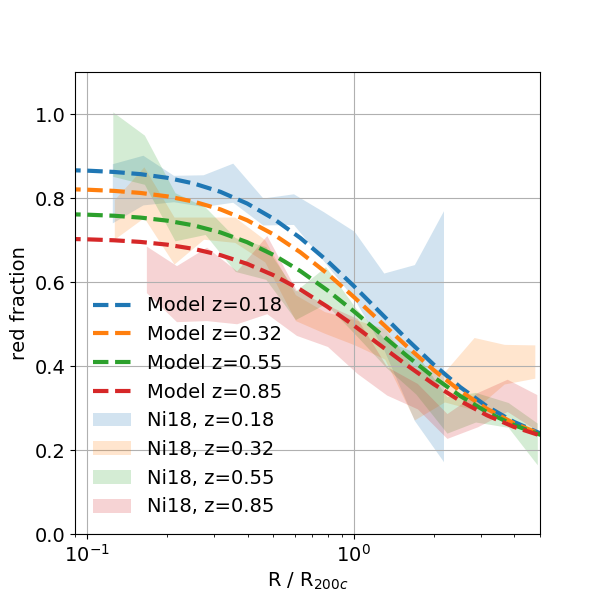
\includegraphics[width=.8\columnwidth]{figures/frac_QU_radius.png}
\caption{\label{fig:SF:QU:fractions:cluster:radius}Fraction of quiescent galaxies as a function of radius of the model compared to the observations of \citep{2018PASJ...70S..24N}.}
\end{figure}

Using this model, we adjust around each cluster the fraction of quiescent galaxies as a function radius. 
We create 10 radial bins of 0.1 R200c width and estimate in each the quiescent fraction. 
We change the is quiescent flag boolean until it matches the fraction desired. 
The choice of the galaxies that see their boolean flag change is random in each radial shell. 
\textcolor{red}{We could follow the values of sSFR to decide which galaxy to change the flag.}

Script :
\begin{verbatim}
    004_3_cluster_red_galaxies.py
\end{verbatim}


\subsection{r-band luminosity function}

Script :
\begin{verbatim}
    004_4_red_sequence.py
\end{verbatim}


We use the cluster galaxy luminosity function from \citet{2018AA...620A..13R} and through an abundance matching procedure 

Finally, using the legacy survey depths maps and masks we update the value of the mask values.

We match in abundance the $V_{max}$ of all (sub) halos within $r_{200c}$ of clusters (or groups) with the optical $r$-band luminosity function of \citet[][Tables 3,5, Eq. 8,9,10]{2018AA...620A..13R}. 
In the abundance matching procedure we introduce a Gaussian scatter of 0.15 dex on the logarithm of $V_{max}$. 
Figs. \ref{fig:optical:LF:MD04}, \ref{fig:optical:LF:MD10} shows the optical luminosity functions obtained in the SMDPL and MDPL2 simulations. 
They align by construction with the \citep{2018AA...620A..13R}. 
Importantly, we see the effect of higher or lower resolution simulations i.e. the number of sub haloes in each cluster or group. 
This effect is dominant at low redshift. 

We bin the cluster catalogue every 0.2 dex in mass to have significant statistics to apply the HAM procedure. 
In each mass bin, we make a realization of the LF.

First we compute the total area to consider :
\begin{equation}
    A = \Sigma_{i \in clusters} \pi  R^2_{200c,i} \; [Mpc^2] ,
\end{equation}
and count the number of galaxies therein ($N_g$). 

The realization of the luminosity is computed as follows. 
The number of galaxies in bins of magnitude 
\begin{equation}
magRange = range(-30, -10, \delta_{mag}), \delta_{mag} = 0.01
\end{equation}
is given by 
\begin{equation}
N_{differential}(m_i) = \Phi(m_i, \bar{z}, \bar{M200c}) \times  A [Mpc^2] \times \delta_{mag} \times \ln(10)
\end{equation}
and the cumulative number  
\begin{equation}
N_{total}(>m_i) = \Sigma^{cumulative}_{m>m_i \in magRange} N_{differential}(m)
\end{equation}

The Ricci 2018 LF is parametrized as follows :
\begin{align}
% Schechter_M_z_M200c
\Phi(mag,z,M200c) & = 0.4 \ln(10) \\ 
\times & 10^{logPhi_{evol}(z, M_\lambda(M200c,z))}    \\
\times & 10^{ 0.4  (m*_{evol}(z, M_\lambda(M200c,z))) - mag) \times (\alpha_{evol}(z, M_\lambda(M200c,z))) + 1)} \\
\times & \exp{( -10^ {( 0.4 * (m*_{evol}(z,M_\lambda(M200c, z)) - mag)))} } \\
\end{align}
with the richness mass relation given by 
\begin{equation}
M_\lambda(M200c, z) = 39.8 * (M200c/3e14)**(0.98) * ((1+z)/(1+0.18))**(-1.08)
\end{equation}
and the redshift evolution of LF parameters are given by Table 3 and Equations 10 and reproduces here :
\begin{equation}
m*_{evol} (z, \lambda) =  - 0.1 \log_{10}(1 + z) - 0.2 \log_{10}(\lambda) - 22
\end{equation}

\begin{equation}
logPhi_{evol} (z, \lambda) =  -0.4 * \log_{10}(1 + z) + 0.8  \log_{10}(\lambda) + 0.3
\end{equation}

\begin{equation}
\alpha_{evol} (z, \lambda) =  -1.3 * \log_{10}(1 + z) + 0.4  \log_{10}(\lambda) - 1.4
\end{equation}


\begin{figure*}
\centering
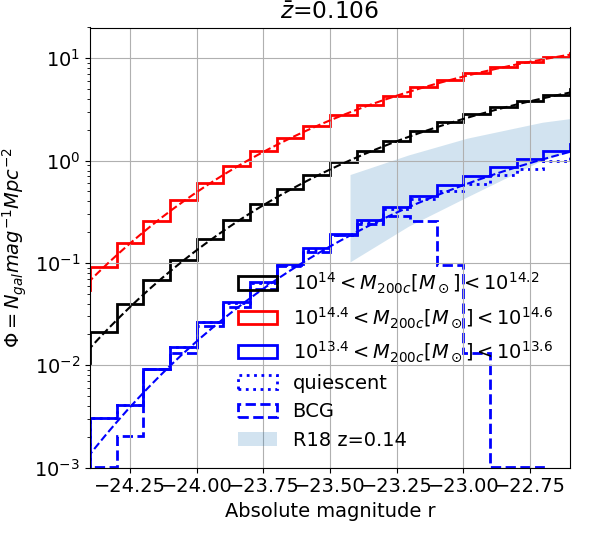
\includegraphics[width=.6\columnwidth,type=png,ext=.png,read=.png]{figures/MD04_cluster_galaxy_LF_z_090430}
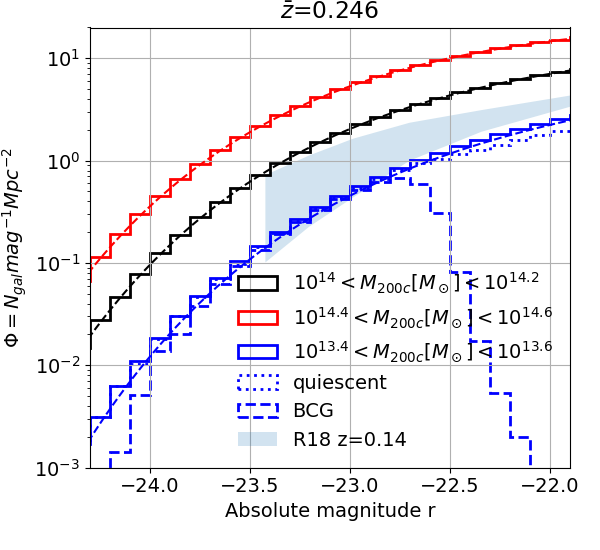
\includegraphics[width=.6\columnwidth,type=png,ext=.png,read=.png]{figures/MD04_cluster_galaxy_LF_z_080230}
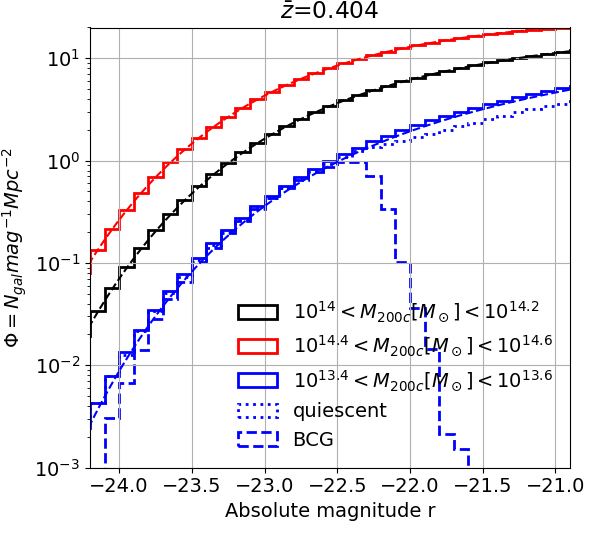
\includegraphics[width=.6\columnwidth,type=png,ext=.png,read=.png]{figures/MD04_cluster_galaxy_LF_z_071240}
\caption{\label{fig:optical:LF:MD04}$r$-band cluster galaxies luminosity function in three redshift bins for SMDPL (high resolution). The high resolution enables to model all galaxies in the cluster.}
\end{figure*}


\begin{figure*}
\centering
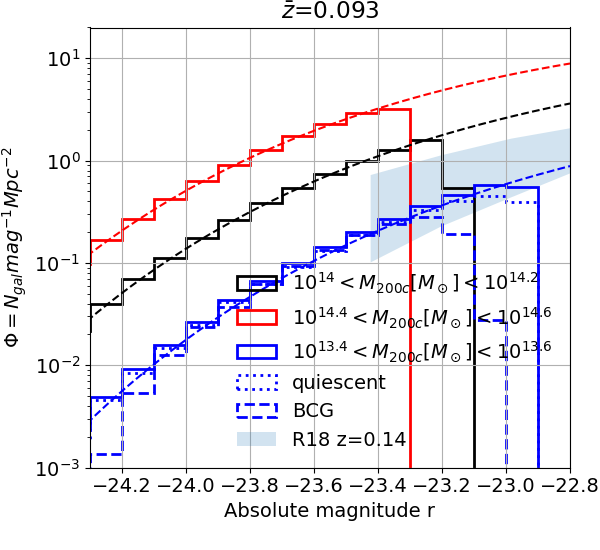
\includegraphics[width=.6\columnwidth,type=png,ext=.png,read=.png]{figures/MD10_cluster_galaxy_LF_z_091520}
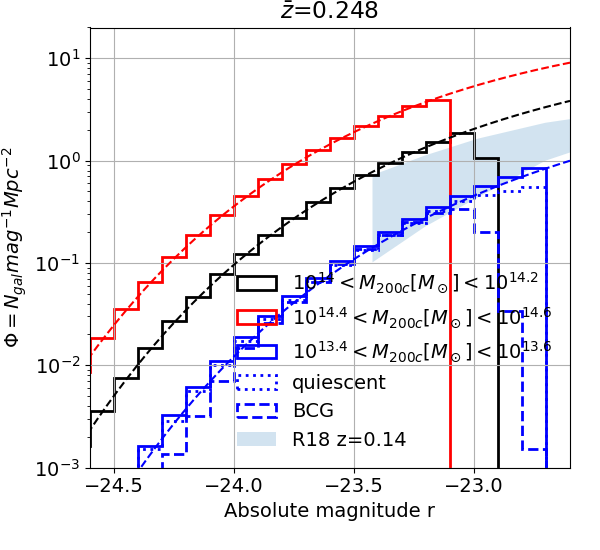
\includegraphics[width=.6\columnwidth,type=png,ext=.png,read=.png]{figures/MD10_cluster_galaxy_LF_z_080130}
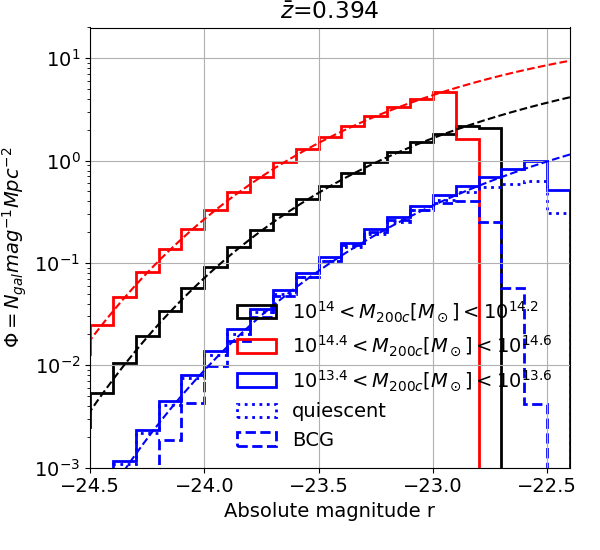
\includegraphics[width=.6\columnwidth,type=png,ext=.png,read=.png]{figures/MD10_cluster_galaxy_LF_z_071730}
%
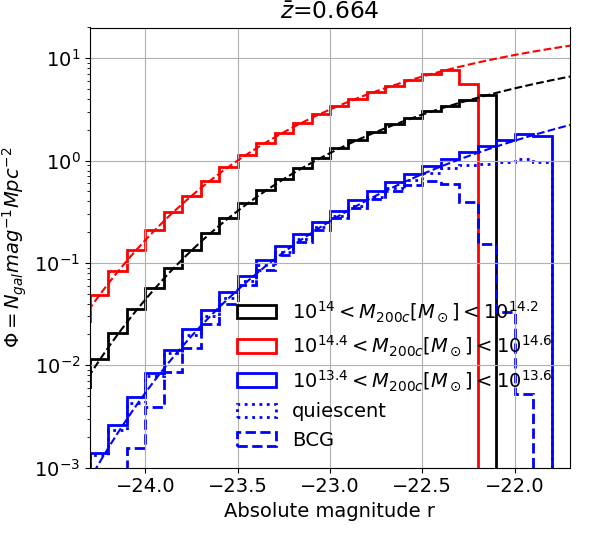
\includegraphics[width=.6\columnwidth,type=png,ext=.png,read=.png]{figures/MD10_cluster_galaxy_LF_z_060080}
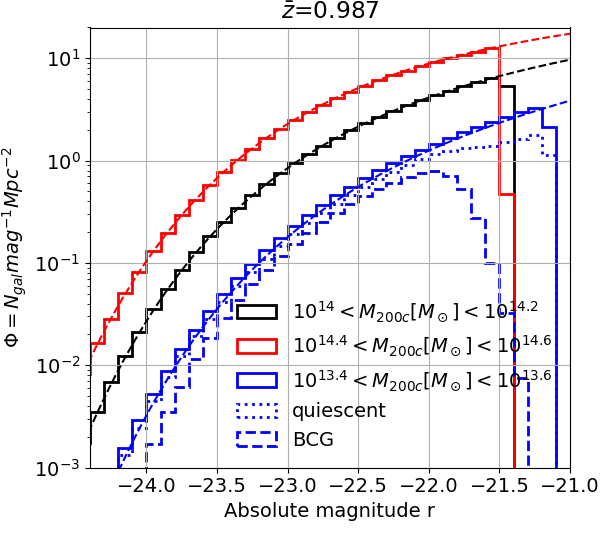
\includegraphics[width=.6\columnwidth,type=png,ext=.png,read=.png]{figures/MD10_cluster_galaxy_LF_z_050320}
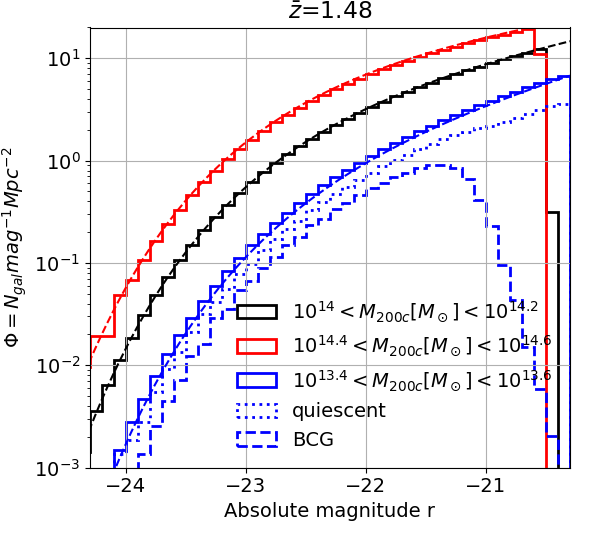
\includegraphics[width=.6\columnwidth,type=png,ext=.png,read=.png]{figures/MD10_cluster_galaxy_LF_z_040320}

\caption{\label{fig:optical:LF:MD10}$r$-band cluster galaxies luminosity function in six redshift bins for MDPL2 (medium resolution). At the lowest redshifts $z<0.3$, resolution is at the limit. }
\end{figure*}

\begin{figure*}
\centering
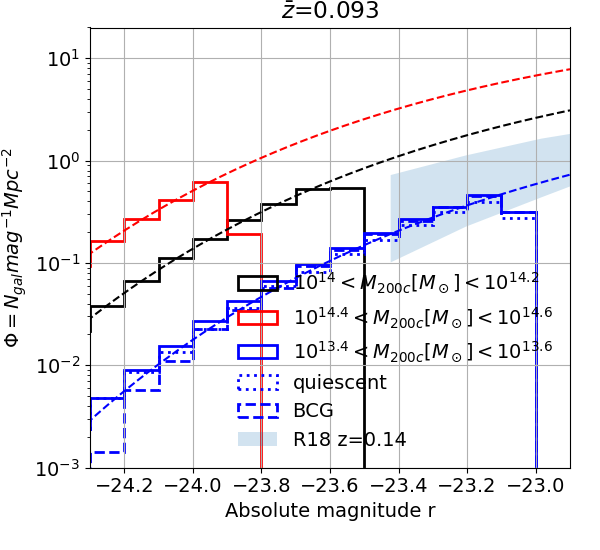
\includegraphics[width=.6\columnwidth,type=png,ext=.png,read=.png]{figures/MD40_cluster_galaxy_LF_z_091520}
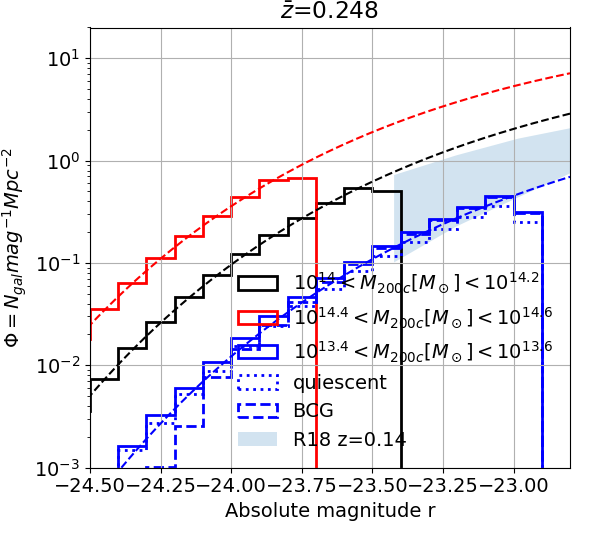
\includegraphics[width=.6\columnwidth,type=png,ext=.png,read=.png]{figures/MD40_cluster_galaxy_LF_z_080130}
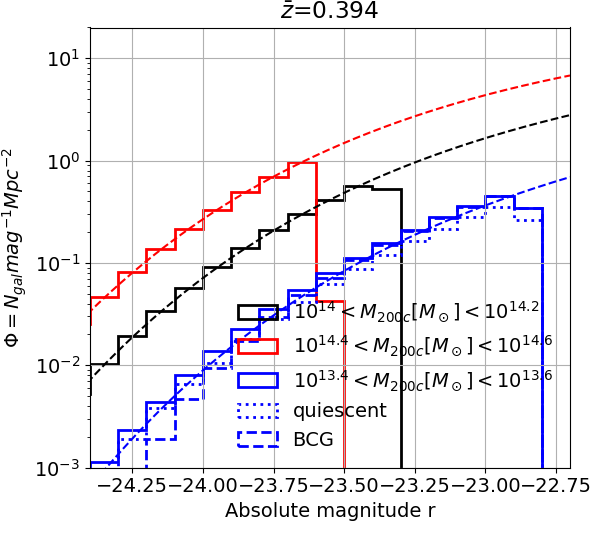
\includegraphics[width=.6\columnwidth,type=png,ext=.png,read=.png]{figures/MD40_cluster_galaxy_LF_z_071730}
%
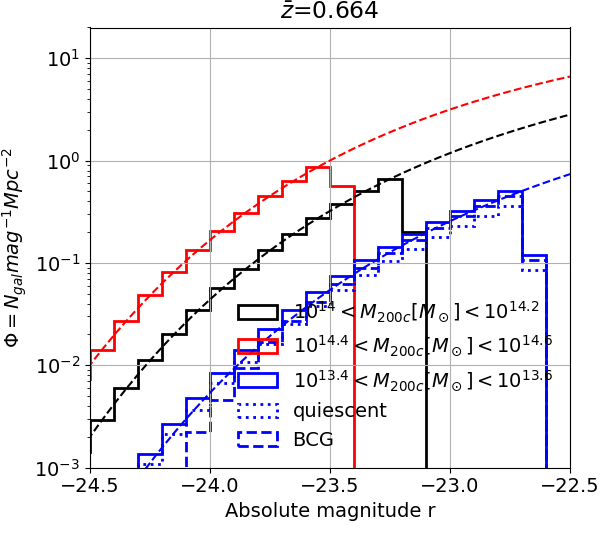
\includegraphics[width=.6\columnwidth,type=png,ext=.png,read=.png]{figures/MD40_cluster_galaxy_LF_z_060080}
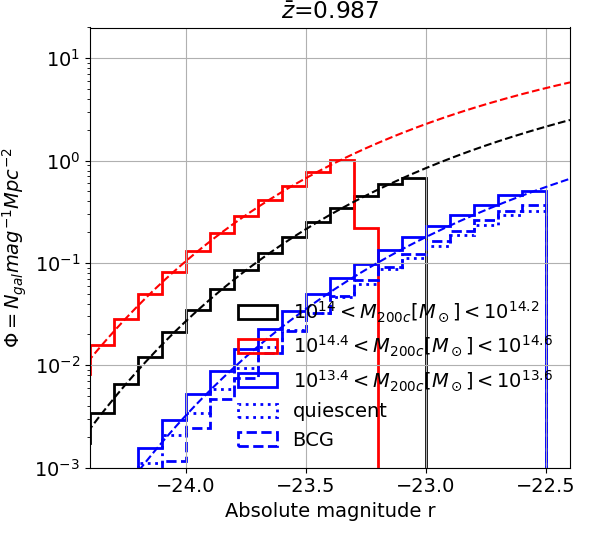
\includegraphics[width=.6\columnwidth,type=png,ext=.png,read=.png]{figures/MD40_cluster_galaxy_LF_z_050320}

\caption{\label{fig:optical:LF:MD40}$r$-band cluster galaxies luminosity function in six redshift bins for HMDPL2 (low resolution). Resolution is clearly lacking to resolve the galaxy population. }
\end{figure*}

\subsection{Observed r, and colors g-r, r-i, i-z}

\textcolor{blue}{VPG: are you using redmapper with parameters fit to reproduce SDSS?}

We use the red sequence as a function of redshift and its scatter to assign observed-frame optical colors to the quiescent galaxies in clusters in the light cones.  
The mean and standard deviation of the colors are obtained with the \textsc{redmapper} software \citep{2014ApJ...785..104R,2015MNRAS.453...38R}. 
We denote them $\bar{c}_{gr}(z)$, $\bar{\sigma}_{gr}(z)$, $\bar{c}_{ri}(z)$, $\bar{\sigma}_{ri}(z)$, $\bar{c}_{iz}(z)$, $\bar{\sigma}_{iz}(z)$. 
For the set of galaxy, we draw a random number following a Gaussian distribution, $N$. 
\begin{equation}
 g-r = \bar{c}_{gr}(z) + N \times \bar{\sigma}_{gr}(z)
\end{equation}
\begin{equation}
 r-i = \bar{c}_{ri}(z) + N \times \bar{\sigma}_{ri}(z)
\end{equation}
\begin{equation}
 i-z = \bar{c}_{iz}(z) + N \times \bar{\sigma}_{iz}(z)
\end{equation}
Using a single random number guarantees that each galaxy has a consistent set of colors with respect to the mean. 
Fig. \ref{fig:optical:RS:model} shows the models used and their scatter. 

\begin{figure}
\centering
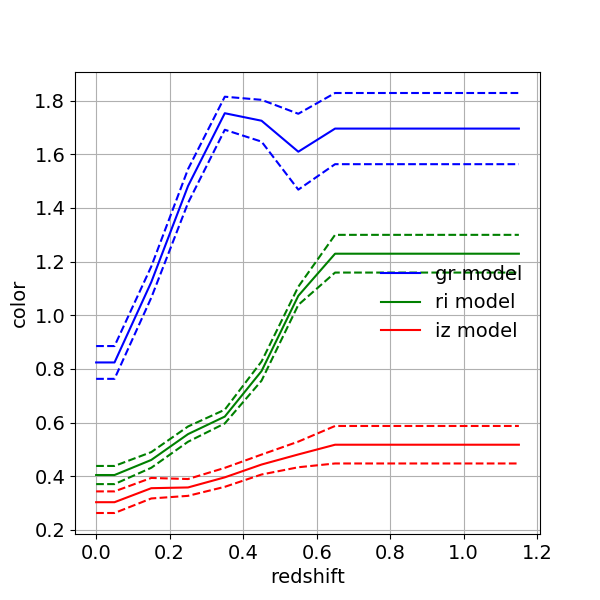
\includegraphics[width=.85\columnwidth,type=png,ext=.png,read=.png]{figures/red_sequence}
\caption{\label{fig:optical:RS:model} Color as a function of redshift of the red sequence galaxies used in this analysis. The solid line represents the mean and the dashed lines the scatter around the mean. }
\end{figure}

We compute the K-correction on the r-band using the g-r color following \citet{2010MNRAS.405.1409C,2012MNRAS.419.1727C}. 
We add the distance modulus and the K-correction to the absolute magnitude in the r band to obtain the observer frame r magnitude. 
We deduce the observed g, i, z magnitudes using the colors obtained before. 
For simplicity, the colors of the star forming population is set to zero, they should be calibrated in a future study, but are not of use in this study. 

We make a realization of the SDSS photometry using the depth maps provided by the \textsc{redmapper} software \citep{2014ApJ...785..104R,2015MNRAS.453...38R}. 
For each galaxy with its position on sky, we extract the 10$\sigma$ depth for the g,r,i,z bands, which we convert into an scatter value on the magnitude. 
The scatter value is multiplied by a random number that follows a Gaussian distribution and added to the observer frame magnitudes to obtain an observed magnitude. 
As uncertainty on the observed magnitude, we report the scatter value extracted from the depth map. 

% \textcolor{red}{start here}
% % We compare to the red sequence observed in HSC \citep{2018PASJ...70S..24N}
% They are compared to the SDSS-IV/SPIDERS observations of red sequence galaxies in X-ray selected clusters \citep{2016MNRAS.463.4490C} as published in the Fourteenth Data Release of the Sloan Digital Sky Survey \citet{SDSS_DR14_2018ApJ23542A}. 
% The agreement is good. 
% 
% \subsection*{Richness}
% 
% We count the number of quiescent glaaxies within $r_{200c}$ and with an absolute magnitude brighter than $M_*+2=-20$ in the r band, to some extent this could be considered as an estimate of the true richness, denoted $N_{200c}$. 
% We fit the slope of the $M_{200c}$ -- $N_{200c}$ and find that depending on the $M_{200c}$ threshold applied the slope fitted will change. 
% When selecting masses larger than $M_{200c}>3\times10^{14}M_\odot$ we find a slope between of $0.8\pm0.2$ compatible with the studies limited to the highest mass clusters: of Saro et al. 2015, Capasso et al. 2019, Ider Chitham et al. 2020. % \citep{2019MNRAS.486.1594C}.
% When selecting masses larger than $M_{200c}>5\times10^{13}M_\odot$  we find slopes between $0.6\pm0.2$ compatible with the studies of Farahi et al. 2016, Baxter et al. 2016, 2018, Simet et al. 2017, McClintock et al. 2018. 
% These studies sample used lower mass clusters than the latter. 
% So we interpret the change in slope measured in these studies as a selection effect and they do not seem incompatible with each other. 
% 
% % The obtained $N_{200c}$ values are within a factor of two from scaling relations between observed richness and mass \citep[e.g.][ and references therein]{2019MNRAS.486.1594C}. 
% SMPDL is very complete and provides god richness estimates. 
% MDPL2 is incomplete in substructure at low redshift. In the range 0.4 to 0.9, the resolution enables a fair representation of scaling relation. 
% The quiescent fraction as a function radius, the lmuminosity function are possibly playing a role there. 
% On top of that, the intrinsic scatter and possible bias between true and observed richness are not very well understood, and this model should be useful to further characterize the ability of red sequence finding algorithms to estimate richness. 

% 
% \section{Studying the performances of the red sequence selection algorithm}
% 
% From the obtained $griz$ magnitudes and SDSS depth maps, we make an SDSS-like (DR8-like) realization of the photometry in the light cones. 
% We inject the simulated red sequence galaxies in the SDSS data, i.e. doubling the number of groups and clusters. 
% We run the \textsc{redMapper}, \textsc{MCMF}, \textsc{AMICO} algorithms and investigate how well input clusters are recovered as a function simulation parameters (halo mass, richness, ...)
% 
% \textcolor{blue}{To be run en of June or so.}
% 
% \subsection{Cluster recovery rate}
% 
% To be done in July
% 
% As a function of many parameters
% 
% \subsubsection{Impact of substructure}
% 
% \subsubsection{Systematics due to the depth maps}
% Give the recovered number density as a function of depth w.r.t. the true number density
% 
% Cluster recovery rates
% 

% \clearpage
\section{Results}
\label{sec:results}

\subsection{Planning the spectroscopic follow-up of eROSITA clusters and their galaxies}

State scientific goals of the survey, refer to the white paper. 

Discuss 4MOST and SDSS-5. \citep{Kollmeier17,Finoguenov2019Msngr}

Give exact numbers for each sub survey component, comment on target selection.

% \subsection{Mass-size relation, fiber magnitudes for SDSS-5 and 4MOST}
% 
% We implement the mass size relation from \citet{2015MNRAS.447.2603L}. 
% The paper is limited to $z<0.1$, so we need another relation for higher redshifts. (Code is below)
% 
% Need to justify the choice of sersic indexes and so on.
% 
% \begin{verbatim}
%  # mass size relation
% 
% # https://arxiv.org/pdf/1411.6355.pdf
% # Table 2 and 3. r mag line for sersic selection
% # equation 2 
% 
% # http://ned.ipac.caltech.edu/level5/March05/Graham/Graham2.html
% b4 = 7.669 
% b1 = 1.678
% f_14_dev = lambda r12 : gammainc(8, b4*(0.7/r12)**(1./6.))
% f_14_exp = lambda r12 : gammainc(2, b1*(0.7/r12)**(1./2.)) # From Raichoor 2017
% f_14_test = lambda r12, nn : gammainc(2, b1*(0.7/r12)**(1./nn)) 
% 
% re_dev = lambda M_star : 0.16*(M_star)**(0.1) * (1+M_star/(2.42*10**(10)))**(0.76-0.1)
% re_exp = lambda M_star : 0.08*(M_star)**(0.16) * (1+M_star/(17.1*10**(10)))**(0.81-0.16)
% # interpolates projected size on the sky
% radius_2_arcsec = interp1d(n.arange(0.00001,6.5,0.001), lc_setup.cosmoMD.arcsec_per_kpc_proper( n.arange(0.00001,6.5,0.001) ).value)
% 
% radius_dev = re_dev(stellar_mass)* radius_2_arcsec(f1['/sky_position/redshift_R'].value[gal][ok])
% radius_exp = re_exp(stellar_mass)* radius_2_arcsec(f1['/sky_position/redshift_R'].value[gal][ok])
% 
% radius = radius_exp
% 
% dm_dev = -2.5*\log_{10}(f_14_dev(radius))
% dm_exp = -2.5*\log_{10}(f_14_exp(radius))
% # initialize the fibermag with the exponential profile
% 
% \end{verbatim}
% \subsection{Fiber collisions}
% 
% Show the 4MOST focal plane and the positioners together with the cluster targets at different redshifts. 
% Take a true cluster from SPIDERS ?
% 
% \subsubsection{Impact on clustering}
% 
% 
% \subsubsection{Impact on dynamical studies}

\subsection{Attempt of direct matching}
We attempt to link each galaxy is to an entry in the \textsc{legacy survey} photometric redshift catalogue \citep{Dey_2019AJ....157..168D,Zou_2019ApJS..242....8Z}. 
We match each simulated galaxy in the light cone to its nearest neighbour in stellar mass (log 10), and redshift (log 10). 
The outcome is not as accurate as we would like when comparing to the luminosity function of galaxies in clusters. 
%We replicate its entry (magnitudes, fluxes, uncertainties, ...). 
%We replace the right ascension and declination fo the true galaxy by that of the simulated galaxy.

\subsection{Cosmological projections}

\textcolor{blue}{NC: here we need to plug in a selection function. Are you planning to test flux limit? count limit? Clerc+18 selection? Or other ?}

We do a cosmological number count experiment where we use directly the true mass of the halos and degrade the redshift information. 
Indeed Pillepich et al. 2018 showed that spectroscopic redshift would bring a boost on the dark energy figure of merit. 
To this aim, we use the software and simulation setup discussed in (Ider Chitham et al 2020)
To degrade the redshift, we draw the redshift uncertainty $\sigma_z = dz/(1+z)$ in a Gaussian of the widths 0.1, 0.05, 0.01, 0.005, 0.001, 0.0005 (6 setups). 
We then fit cosmological parameters while varying the width of redshift bins : 0.2, 0.1, ... 0.0005 (7 binning schemes). 
We obtain a total uncertainty on the reduced $\Omega_m^p \times \sigma_8^q$ parameter (or the area of the contour ?) for the 6x7=42 setups. 
We represent on Fig. XX %\ref{fig:cosmo:dz:bins} 
this accuracy parameter w.r.t. the perfect fit using redshifts (with the lne of sight velocity projected).

We find that for a given redshift accuracy, the optimal binning width is N times the redshift accuracy. 

We find that obtaining spectroscopic redshifts is key to retrieve maximal cosmological information when doing a number count experiment. 
Indeed, there is a factor of XX improvement when changing from photometric redshifts from spectroscopic redshifts. 
% This finding is similar to the results of Pillepich et al. 2018. 

\subsection{Other result}

\subsection{Another result}

\section*{Acknowledgements}
J. Comparat thanks XXXXX

The CosmoSim database is a service of the Leibniz-Institute for Astrophysics Potsdam (AIP).
The MultiDark database was developed in cooperation with the Spanish MultiDark Consolider Project CSD2009-00064.

This project made use of 
\textsc{gawk}\footnote{{https://www.gnu.org/software/gawk/}}, 
\textsc{python}3\footnote{\url{https://www.python.org}}, 
\textsc{astropy} \citep{Astropy2013AA, Astropy2018AJ}, 
\textsc{topcat/stilts}\footnote{\url{http://www.star.bris.ac.uk/~mbt/stilts/}} \citet{2006ASPC..351..666T}, 
\textsc{slurm}\footnote{\url{https://slurm.schedmd.com/publications.html}}, 
the ``K-corrections calculator''service \footnote{\url{http://kcor.sai.msu.ru/}}, 
...

%%%%%%%%%%%%%%%%%%%%%%%%%%%%%%%%%%%%%%%%%%%%%%%%%%
%%%%%%%%%%%%%%%%%%%% REFERENCES %%%%%%%%%%%%%%%%%%
\bibliographystyle{mnras}
\bibliography{references}

%%%%%%%%%%%%%%%%%%%%%%%%%%%%%%%%%%%%%%%%%%%%%%%%%%
%%%%%%%%%%%%%%%%% APPENDICES %%%%%%%%%%%%%%%%%%%%%
 
\appendix

\section{galaxies}
\bsp	% typesetting comment
\label{lastpage}
\end{document}



We split, in a statistical manner, the star forming from the quiescent galaxies using the COSMOS catalog \citep{Ilbert2013AA556A55I}, where star forming galaxies (SF) are selected with a $\log_{10}$ of their specific star formation rate greater than -11. 
%The COSMOS catalogue includes a complete census of the galaxy population as a function of their environment up to redshift four. 

\textcolor{blue}{VGP: I usually use Franx+2008 cut for model, sSFR (Gyr-1) >0.3/tHubble, which is based on observations that suggest that the split for SF/quiescent varies w z (this is also seen in models). Thus, I'll like to see a comparison w this or at least a discussion.}

The rest of the population is considered as quiescent (QU). 
We fit the fraction of SF and QU galaxies as a function of mass and redshift. 
The data points used and fitted curves obtained are shown on Fig. \ref{fig:SF:QU:cosmos}
We obtain the following parametrization. 

\begin{equation}
 f_{QU} (\log_{10}(M),z) = 0.5+0.5 \epsilon\left(\frac{\log_{10}(M) - \log_{10}(M0(z)) }{ \sigma_0(z)} \right)
 \label{eqn:qu:fraction}
\end{equation}
where 
\begin{equation}
 \log_{10}(M0(z)) = 9.71 + 0.78 (1+z)
\end{equation}
and 
\begin{equation}
 \sigma_0(z) = 1.54 - 0.45 (1+z)
\end{equation}

and $\epsilon$ is the Gauss error function 
\begin{equation}
\label{eqn:gauss:err:fct}
\epsilon(x)=\frac{2}{\sqrt{{\rm \pi}}}\int_{t=0}^{t=x} {\rm e}^{-t^2}\,dt
\end{equation}

We draw one random number per galaxy, denoted $\mathcal{R}$. 
It is uniformly distributed between 0 and 1. 
We use it to assign its state star-forming or quiescent. 
For each galaxy we evaluate $f_{QU} (log_{10}(M),z) $ using Eq. (\ref{eqn:qu:fraction}) and compare it to the random number. 
If $\mathcal{R}>f_{QU} (log_{10}(M),z)$, then the galaxy is star-forming, else it is quiescent. 

\begin{figure}
\centering
%\includegraphics[width=.85\columnwidth,type=png,ext=.png,read=.png]{/home/comparat/software/lss_mock_dev/figures/galaxies/SFR/summary_mass-redshift-SSFRm11cut_hist_fractionQU}
\caption{\label{fig:SF:QU:cosmos} Fraction of quiescent galaxies as a function of mass and redshift. 
}
\end{figure}

For the star-forming galaxies, we compute star formation rates (SFR) following the main sequence from \citet[][Eq. 1,2,3]{2012ApJ...754L..29W} with a scatter of 0.34 dex.
\begin{equation}
\overline{\log_{10}(SFR)} (\log_{10}(M),z)= (0.70 - 0.13 z) (\log_{10}(M) - 10.5 ) + 0.38 + 1.14 z - 0.19 z^2
\label{eqn:SFSEQ:SF:mean}
\end{equation}
\begin{equation}
 \log_{10}(SFR) (\log_{10}(M),z) = \overline{\log_{10}(SFR)} (\log_{10}(M),z) + \mathcal{N}(0, 0.34)
\label{eqn:SFSEQ:SF}
\end{equation}

For the quiescent, we fit a SF sequence on the COSMOS data as well as its scatter
\begin{equation}
\overline{\log_{10}(SFR)} (\log_{10}(M),z)= (1.43 - 0.57 z )\log_{10}(M) - 16.26 + 6.32 z 
\label{eqn:SFSEQ:QU:mean}
\end{equation}
\begin{equation}
 \sigma_1 (z) : 0.99 -0.34 z
\end{equation}
\begin{equation}
 \log_{10}(SFR) (\log_{10}(M),z) = \overline{\log_{10}(SFR)} (\log_{10}(M),z) + \mathcal{N}(0, \sigma_1 (z) )
\label{eqn:SFSEQ:QU}
\end{equation}

Fig. \ref{fig:SF:sequence} shows the star formation rate vs. stellar mass for the two populations as well as the mean relations given in Equations \ref{eqn:SFSEQ:SF:mean},  \ref{eqn:SFSEQ:QU:mean}.  


\begin{figure*}
\centering
%\includegraphics[width=.45\columnwidth,type=png,ext=.png,read=.png]{/home/comparat/software/lss_mock_dev/figures/galaxies/SFR/mass-SFR-SSFRm11cut_z_0.3}
%\includegraphics[width=.45\columnwidth,type=png,ext=.png,read=.png]{/home/comparat/software/lss_mock_dev/figures/galaxies/SFR/mass-SFR-SSFRm11cut_z_0.5}
%\includegraphics[width=.45\columnwidth,type=png,ext=.png,read=.png]{/home/comparat/software/lss_mock_dev/figures/galaxies/SFR/mass-SFR-SSFRm11cut_z_0.7}
%\includegraphics[width=.45\columnwidth,type=png,ext=.png,read=.png]{/home/comparat/software/lss_mock_dev/figures/galaxies/SFR/mass-SFR-SSFRm11cut_z_0.9}
\caption{\label{fig:SF:sequence}
Star formation rate v.s stellar mass for the SF and QU populations. 
The red line shows the star formation main sequence from \citep{2012ApJ...754L..29W}. 
The green line shows the fit to the QU population. 
}
\end{figure*}



\subsection{AGN}
We then populate or `paint' the halos with properties. 
For AGNs, we follow \citep{2018MNRAS.tmp.3272G,2019MNRAS.tmp.1335C} without a prior on the fraction of satellites i.e. we treat all satellites haloes in the simulation as if they were distinct haloes. 
% We describe the clusters and their X-ray flux in a very simple manner in see Sec. \ref{sec:X:cluster:model}. 
% We intend to do a full comparison of X-ray painting models in a future study. 
% We describe the galaxies around and within in see Sec. \ref{sec:optical:cluster:model}.


%\subsubsection{Stellar mass and star formation rate}
%\label{subsec:M:SFR}
%For each halo and subhalo we compute a stellar mass using an evolving stellar mass to halo mass relation \citep{2013MNRAS.428.3121M}. 
% The logarithm of the stellar masses are drawn from a Gaussian distribution (with scatter 0.15 dex) around a mean obtained with Eq. \ref{eqn:SMHMR}. 
% \begin{equation}
% \label{eqn:SMHMR}
%  \bar{M}^*(M_h, z) = \frac{A(M_H,z)}{B(M_h,z) + C(M_h,z)} 
% \end{equation}
% where $M_h=M_{vir}$ and 
% \begin{align*}
% & A(M_h,z) = 4 M_h \left(0.0351 - 0.0247 \frac{z}{1+z}\right) \\
% & B(M_h,z) = \left(\frac{M_h}{10^{11.59 + 1.195  \frac{z}{1+z} } } \right)^{- 1.376 + 0.826  \frac{z}{1+z}} \\
% & C(M_h,z) = \left( \frac{M_h }{10^{11.59 + 1.195 \frac{z}{1+z}} }\right)^{0.608 + 0.329 \frac{z}{1+z}}.
% \end{align*}
% 
%The obtained mass functions are in good agreement with data, see Fig. 2 of \citet{2019MNRAS.tmp.1335C}. 


For each halo and subhalo we compute a stellar mass using an evolving stellar mass to halo mass relation \citep{2013MNRAS.428.3121M}. 
It produces stellar mass functions in fair agreement with COSMOS observations \citep[][, Fig. 5]{Ilbert2013AA556A55I}, e.g. see Fig. 2 of \citet{2019MNRAS.tmp.1335C}. 
